\section{SSLStrip+}

%%%%%%%%%%%%%%%%%%%%%%%%%%%%%%%%%%%%
% HSTS                             %
%%%%%%%%%%%%%%%%%%%%%%%%%%%%%%%%%%%%
\begin{frame}{Fonctionnement de HSTS}
  \begin{columns}
    \begin{column}{0.6\textwidth}
      \begin{exampleblock}{HTTP Strict Transport Security}
        \begin{itemize}
        \item RFC 6797
        \item Entête HTTP 'Strict-Transport-Security'
        \item Date d'expiration
        \end{itemize}
      \end{exampleblock}

      \begin{alertblock}{Problème}
        \begin{itemize}
        \item Ne protège pas la première connexion
        \end{itemize}
      \end{alertblock}

      \begin{block}{Solution}
        \begin{itemize}
        \item HSTS preload
        \end{itemize}
      \end{block}

    \end{column}
    \begin{column}{0.4\textwidth}
      \begin{figure}
        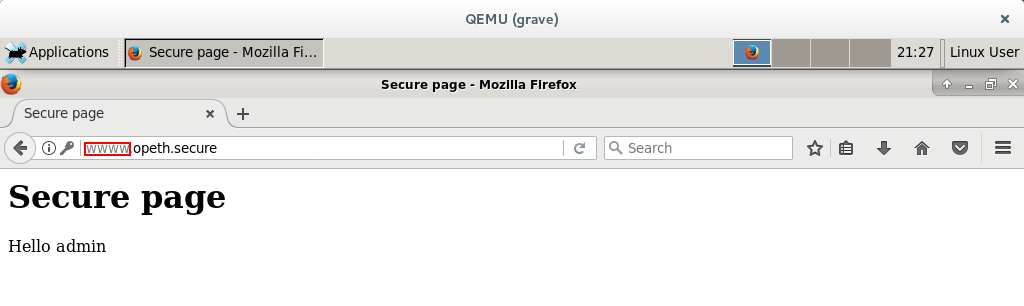
\includegraphics[width=\linewidth]{../medias/sslstrip2/screen2.png}
      \end{figure}
      \begin{figure}
        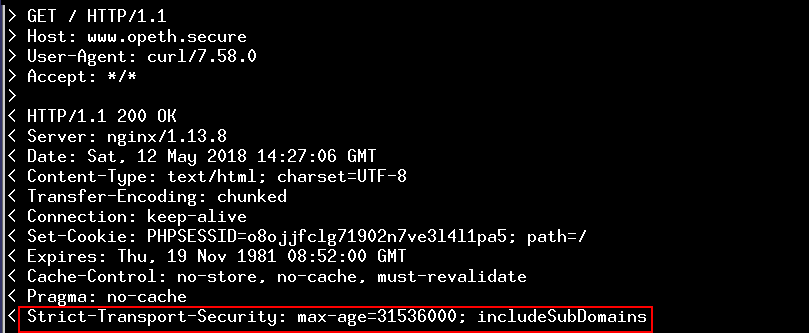
\includegraphics[width=\linewidth]{../medias/hsts.png}
      \end{figure}
    \end{column}
  \end{columns}

\end{frame}

%%%%%%%%%%%%%%%%%%%%%%%%%%%%%%%%%%%%
% SSLstrip+                        %
%%%%%%%%%%%%%%%%%%%%%%%%%%%%%%%%%%%%

\begin{frame}[fragile]{Attaque SSLStrip+}
  \begin{columns}
    \begin{column}{0.7\textwidth}
      \begin{block}{Principes}
        \begin{itemize}
        \item{Attaquer le trafic DNS}
        \item{Utiliser un faux nom de domaine}
        \item{Remplacer les URL sécurisées par le faux nom}
        \end{itemize}
      \end{block}
    \end{column}
    \begin{column}{0.3\textwidth}
    \begin{exampleblock}{Outil }
      \begin{itemize}
      \item{Dnsmasq}
      \end{itemize}
    \end{exampleblock}

    \end{column}
  \end{columns}
  \begin{figure}
    Remplacement des liens HTTP :
    \begin{minted}{python}
def __replace_https_to_http(self, data):
    return re.sub(b'https://' + bytes(FORWARD_HOST_HSTS), b'http://' + bytes(FAKE_HOST), data)
        \end{minted}
        Modification de l'entête 'Host' :
        \begin{minted}{python}
def __replace_host(self, data):
    return re.sub(b'Host: ' + bytes(FAKE_HOST), b'Host: ' + bytes(FORWARD_HOST_HSTS), data)
        \end{minted}
      \end{figure}

\end{frame}

\begin{frame}{Attaque SSLStrip+}
  \begin{figure}
    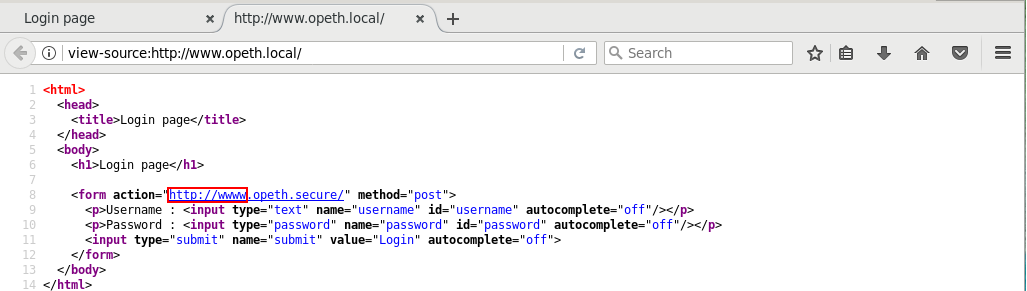
\includegraphics[width=1.0\linewidth]{../medias/sslstrip2/screen5-2.png}
  \end{figure}

  \begin{figure}
    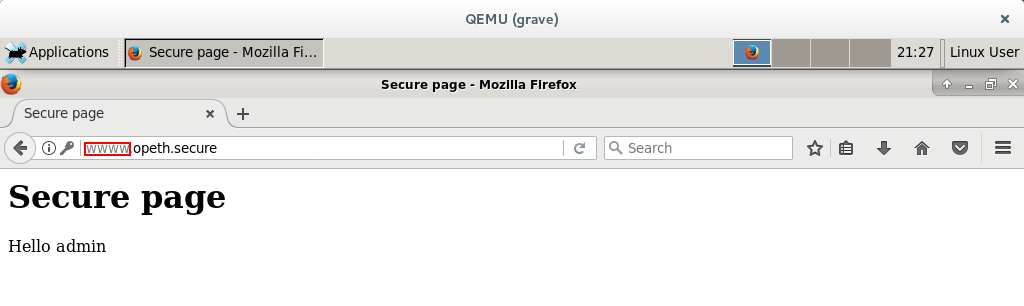
\includegraphics[width=1.0\linewidth]{../medias/sslstrip2/screen6.png}
  \end{figure}

\end{frame}

%%%%%%%%%%%%%%%%%%%%%%%%%%%%%%%%%%%%
% SSLStrip+ overview               %
%%%%%%%%%%%%%%%%%%%%%%%%%%%%%%%%%%%%

\begin{frame}{Attaque SSLStrip+}
    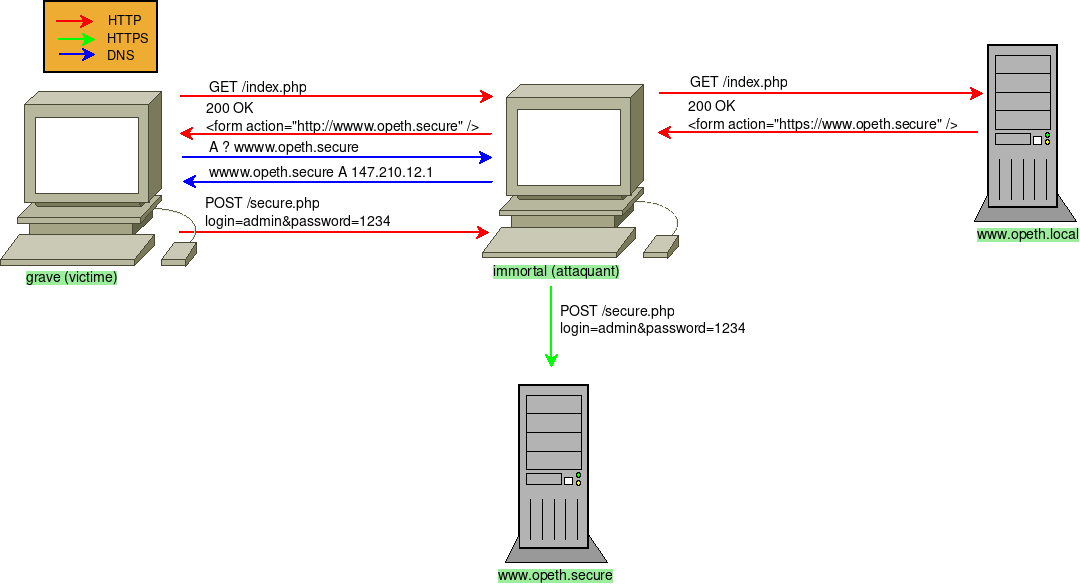
\includegraphics[width=\linewidth]{../medias/sslstrip2/attack.png}
\end{frame}
